\documentclass[10pt,a4paper]{article}
\usepackage[a4paper,vmargin={30mm},hmargin={30mm}]{geometry}
\usepackage[utf8x]{inputenc}
\usepackage{ucs}
\usepackage{amsmath}
\usepackage{amsfonts}
\usepackage{amssymb}
\usepackage{parskip} % Skip indentation of first row
\usepackage{graphicx} % Graphics support
\usepackage{longtable} % Tables across several pages
\author{Danilo Bargen\\http://ich-wars-nicht.ch/}
\title{Theoriesammlung Analysis 1}

\begin{document}

\begin{titlepage}
	\maketitle
	\vspace{120mm}
	\center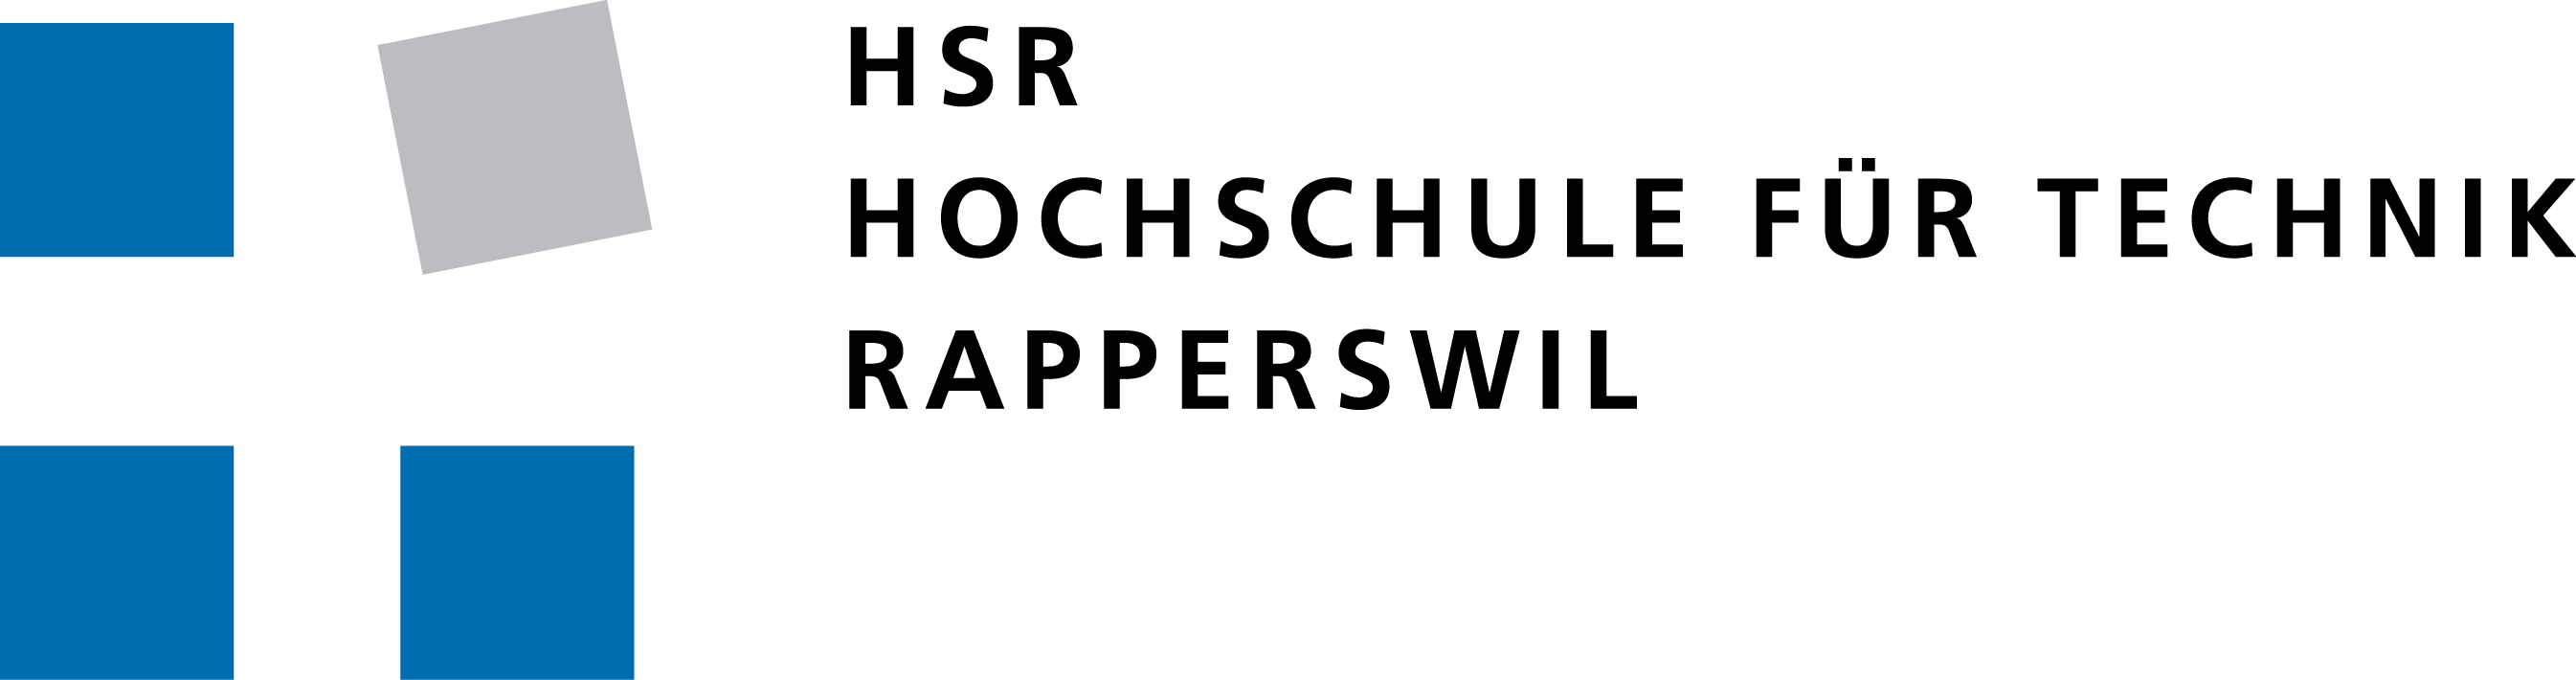
\includegraphics{hsr_logo.png}
	\thispagestyle{empty} % Don't start page numbers on this page
\end{titlepage}

\tableofcontents\newpage

\section{Funktionen}

\subsection{Gerade, ungerade und periodische Funktion}

Die Funktion $f$ heisst

\begin{itemize}
\item \textit{gerade}, wenn
$$\forall x \in DB(f): f(-x) = f(x)$$
\item \textit{ungerade}, wenn
$$\forall x \in DB(f): f(-x) = -f(x)$$
\item \textit{periodisch} mit der Periode $p$, wenn
$$\forall x \in DB(f): f(x + p) = f(x)$$
Die kleinste positive Periode heisst \textit{primitive Periode}.
\end{itemize}


\subsection{Umkehrbarkeit}

Die Funktion $f$ heisst \textit{umkehrbar}, wenn
$$(f(x_1) = f(x_2) \Rightarrow x_1 = x_2$$

\subsection{Allgemeine Gleichungsregel}

Für jede umkehrbare Funktion $f$ gilt: Man darf beidseitig einer Funktion dieselbe umkehrbare Funktion anwenden, wenn beide Seiten in ihrem Definitionsbereich liegen. Mathematisch ausgedrückt:
$$\forall x_1, x_2 \in DB(f): x_1 = x_2 \Leftrightarrow f(x_1) = f(x_2)$$


\subsection{Gleichungsregel für das Wegschaffen von Wurzeln}

Um die Wurzel auf der linken Seite der Gleichung
$$\sqrt{R} = S$$
wegzuschaffen, sind zwei Fälle zu unterscheiden:

\begin{itemize}
\item Wenn $S \geq 0$ ist, so ist die Gleichung äquivalent zu $R = S^2$
\item Wenn $S < 0$ ist, ist die Gleichung unerfüllbar.
\end{itemize}

oder auf eine kurze Formel gebracht:
$$\sqrt{R} = S \Leftrightarrow R = S^2 \wedge S \geq 0$$


\subsection{Monotone Funktionen}

\begin{itemize}
	\item Sei $f$ eine monoton steigende Funktion. Dann gilt
	$$f(x_1) < f(x_2) \Rightarrow x_1 < x_2$$

	\item Ist aber $f$ eine monoton fallende Funktion, so gilt
	$$f(x_1) < f(x_2) \Rightarrow x_1 > x_2$$
\end{itemize}


\subsection{Allgemeine Ungleichungsregel}

Für jede streng monoton steigende Funktion $f$ gilt: Man darf beidseitig einer Ungleichung dieselbe streng monoton steigende Funktion anwenden, wenn beide Seiten in ihrem Definitionsbereich liegen. Oder mathematisch ausgedrückt:
$$\forall x_1, x_2 \in DB(f): x_1 < x_2 \Leftrightarrow f(x_1) < f(x_2)$$

Ferner gilt für jede streng monoton fallende Funktion $f$: Man darf beidseitig einer Ungleichung dieselbe streng monoton fallende Funktion anwenden, wenn beide Seiten in ihrem Definitionsbereich liegen. Dabei ist aber des Vergleichszeichen umzudrehen. Mathematisch ausgedrückt:
$$\forall x_1, x_2 \in DB(f): x_1 < x_2 \Leftrightarrow f(x_1) > f(x_2)$$


\subsection{Arithmetische Grundoperationen mit Funktionen}

$f$ und $g$ seien reelle Funktionen. Dann sind folgende Operationen definiert:
\begin{itemize}
\item $\displaystyle -f := x \mapsto -f(x)$
\item $\displaystyle f + g := x \mapsto f(x) + g(x)$
\item $\displaystyle f - g := x \mapsto f(x) - g(x)$
\item $\displaystyle f \cdot g := x \mapsto f(x) \cdot g(x)$
\item $\displaystyle \frac{f}{g} := x \mapsto \frac{f(x)}{g(x)}$
\end{itemize}

Beim Vorzeichenwechsel ist der Defintionsbereich identisch mit jenem von $f$. Bei Summe, Differenz und Produkt ist er gleich dem Durchschnitt der Definitionsbereiche von $f$ und $g$ und im Falle des Quotienten darf $g$ natürlich nicht den Wert $0$ haben; er ist daher gleich $\displaystyle (DB(f) \cap DB(g)) \ \{x|g(x) = 0\}$.

Sei ferner $c$ eine Zahl. Dann sind folgende Funktionen definiert:

\begin{itemize}
\item $\displaystyle (f + c) := x \mapsto f(x) + c$
\item $\displaystyle (f - c) := x \mapsto f(x) - c$
\item $\displaystyle (c - f) := x \mapsto c - f(x)$
\item $\displaystyle (f \cdot c) := x \mapsto f(x) \cdot c$
\item $\displaystyle \frac{f}{c} := x \mapsto \frac{f(x)}{c} \textrm{ für } c \neq 0$
\item $\displaystyle \frac{c}{f} := x \mapsto \frac{c}{f(x)}$
\end{itemize}

Im letzten Fall ist der Definitionsbereich gleich $DB(f) \ \{x|f(x) = 0 \}$, in den übrigen Fällen ist er identisch mit jenem von $f$.


\subsection{Verkettung oder Komposition}

Gegeben seien die Funktionen $f$ und $g$. Dann nennt man die Funktion
$$x \mapsto f(g(x))$$
die \textit{Verkettung} oder \textit{Komposition} der Funktionen $f$ und $g$. Man bezeichnet sie mit
$$f \circ g$$
und liest das als \textit{$f$ nach $g$}.


\subsection{Graphen der Verkettung von Funktionen mit linearen Funktionen}

Der Graph der Funktion $f$ sei bekannt. Dann geht der Graph der Funktion
$$x \mapsto af(x) + b$$
aus jenem von f durch folgende geometrische Operationen hervor (Reihenfolge wesentlich!)
\begin{enumerate}
	\item Vertikale Skalierung um den Faktor $|a|$
	\begin{itemize}
		\item Wenn $a < 0$ zusätzlich eine Spiegelung an der 1. Koordinatenachse
	\end{itemize}
	\item Vertikalverschiebung um $|b|$ und zwar
	\begin{itemize}
		\item Nach oben, wenn $b > 0$
		\item Nach unten, wenn $b < 0$
	\end{itemize}
\end{enumerate}

Ferner geht der Graph der Funktion
$$x \mapsto f(ax + b)$$
aus jenem $f$ durch folgende geometrische Operationen hervor (Reihenfolge wesentlich!)
\begin{enumerate}
	\item Horizontalverschiebung um $|b|$ und zwar
	\begin{itemize}
		\item Nach links, wenn $b > 0$
		\item Nach rechts, wenn $b < 0$
	\end{itemize}
	\item Horizontale Skalierung um den Faktor $\displaystyle\frac{1}{|a|}$
	\begin{itemize}
		\item Wenn $a < 0$ zusätzlich eine Spiegelung an der 2. Koordinatenachse	
	\end{itemize}
\end{enumerate}


\subsection{Umkehrfunktion}

Sei $f$ eine umkehrbare Funktion. Dann heisst die Funktion $f^{–1}$, für welche gilt
$$f^{-1}(y) = x \Leftrightarrow y = f(x)$$
die \textit{Umkehrfunktion} von $f$. Für termdefinierte Funktionen gilt also
$$f = x \mapsto y \Leftrightarrow f^{-1} = y \mapsto x$$
In anderen Worten: Bei der Umkehrfunktion werden einfach die Rollen von Argument und Funktionswert vertauscht. Dies läuft auf eine Spiegelung des Graphen der gegebenen Funktion an der ersdten Quadrantenhalbierenden hinaus.


\subsection{Graphen von Umkehrfunktionen}

Sei $f$ eine umkehrbare Funktion. Dann ist der Graph von $f^{-1}$ das Spiegelbild des Graphen von $f$ an der 1. Quadrantenhalbierenden.


\subsection{Verkettung einer Funktion mit ihrer Umkehrfunktion}

Sei $f$ eine umkehrbare Funktion. Dann gilt
$$\forall x \in DB(f): f^{-1}(f(x)) = x$$
oder knapper
$$f^{-1} \circ f = id_{DB(f)}$$

% definition 10

% definition 11

% ... todo

\section{Differentialrechnung}

\subsection{Ableitung}

$f$ sei eine reelle Funktion und $x$ ein Argument. Wenn der Grenzwert
$$f'(x) = \lim_{\Delta x \to 0}\frac{f(x + \Delta x) - f(x)}{\Delta x}$$
im eigentlichen Sinne existiert, so heisst die Funktion $f$ an der Stelle $x$ \textit{differenzierbar} und der Grenzwert heisst die \textit{Ableitung} von $f$ an der Stelle $x$.

In physikalischen und technischen Anwendungen treten häufig Funktionen auf, in denen das Argument die Zeit $t$ bedeutet. In diesem Fall hat es sich eingebürgert, die Ableitung mit einen über das Funktionssymbol geschriebenen Punkt zu bezeichnen, also
$$\dot{f}(t) \textrm{ statt } f'(t)$$


\subsection{Wichtige Ableitungsfunktionen}

\renewcommand{\arraystretch}{1.8}
\begin{longtable}{ll}
\hline
\textbf{Funktion} & \textbf{Ableitungsfunktion} \\\hline\endhead
$x \mapsto 1$ & $x \mapsto 0$ \\
$id := x \mapsto x$ & $x \mapsto 1$ \\
$sqr := x \mapsto x^2$ & $x \mapsto 2x$ \\
$rez := x \mapsto \frac{1}{x}$ & $x \mapsto -\frac{1}{x^2}$ \\
$sqrt := x \mapsto \sqrt{x}$ & $x \mapsto \frac{1}{2\sqrt{x}}$ \\
$x \mapsto x^n$ & $x \mapsto nx^{n-1}$ \\
$exp := x \mapsto e^x$ & $x \mapsto e^x$ \\
$x \mapsto e^{-x}$ & $x \mapsto -e^{-x}$ \\
$ln$ & $x \mapsto \frac{1}{x} \textrm{ für } x > 0$ \\
$sin$ & $cos$ \\
$cos$ & $-sin$ \\
$tan$ & $1 + tan^2 = \frac{1}{cos^2}$ \\
$arcsin$ & $\frac{1}{\sqrt{1 - x^2}}$ \\
$arccos$ & $-\frac{1}{\sqrt{1 - x^2}}$ \\
$arctan$ & $\frac{1}{1 + x^2}$ \\
\end{longtable}

\subsection{Linearitätsregeln für die Ableitung}

$f$ und $g$ seien differenzierbare Funktionen und $c$ eine Konstante. Dann gelten
diese beiden sogenannte \textit{Linearitätsregeln}
\begin{itemize}
	\item $(f + g)' = f' + g'$
	\item $(c \cdot f)' = c \cdot f'$
\end{itemize}

Wenn die Fuktionen durch Terme $S$ und $T$ definiert sind, so kann man die Regeln auch auf die Terme übertragen:
\begin{itemize}
	\item $\displaystyle\frac{d}{dx}(S + T) = \frac{dS}{dx} + \frac{dT}{dx}$
	\item $\displaystyle\frac{d}{dx}(c \cdot T) = c \cdot \frac{dT}{dx}$
\end{itemize}


\subsection{Produkt- und Quotientenregel für Ableitungen}

$f$ und $g$ seien differenzierbare Funktionen. Dann ist
\begin{itemize}
	\item $\displaystyle(f \cdot g)' = f' \cdot g + f \cdot g'$
	\item $\displaystyle\left(\frac{f}{g}\right)' = \frac{f' \cdot g - f \cdot g'}{g^2}$
\end{itemize}

Wenn die Funktionen mit Hilfe von Zuordnungstermen $S$ und $T$ definiert sind, so lassen sich diese Regeln auf die Terme übertragen.
\begin{itemize}
	\item $\displaystyle\frac{d}{dx}(S \cdot T) = \left(\frac{dS}{dx}\right)T + S\left(\frac{dT}{dx}\right)$
	\item $\displaystyle\frac{d}{dx}\left(\frac{S}{T}\right) = \frac{\displaystyle\left(\frac{dS}{dx}\right)T - S\left(\frac{dT}{dx}\right)}{T^2}$
\end{itemize}


\subsection{Kettenregel für Ableitungen}

$f$ und $g$ seien differenzierbare Funktionen. Dann ist die Ableitung ihrer Verkettung an der Stelle $x$ gegeben durch
$$(f \circ g)'(x) = f'(g(x))g'(x)$$
oder in der Termschreibweise
$$\frac{d}{dx}f(g(x)) = f'(g(x)) \cdot \frac{d}{dx}g(x)$$
Wenn wir beachten, dass $f'(g(x)) = (f' \circ g)(x)$ ist, bekommen wir für die Ablei-
tungsfunktion
$$(f \circ g)' = (f' \circ g) \cdot g'$$


\subsection{Linearisierungsformel}

$f$ sei eine an der Stelle $x_0$ differenzierbare Funktion. Dann ist der Graph der Funktion
$$T := x \mapsto f'(x_0)(x-x_0) + f(x_0)$$
die Tangente an den Graphen von $f$ im Punkt $(x_0, f(x_0))$.

Der Ausdruck $x - x_0$ kann auch als $\Delta x$ geschrieben werden.


\subsection{Algorithmus von Newton}

Wir betrachten die Gleichung
$$f(x) = 0$$
$x_0$ sei eine Schätzung für die exakte Lösung $x^*$. Die Funktion $f$ sei zwischen $x_0$ und $x^*$ differenzierbar.

Dann strebt die durch die Vorschrift
$$x_{n+1} = x_n - \frac{f(x_n)}{f'(x_n)}$$
konstruierte Folge unter gewissen, hier nicht näher präzisierten Bedingungen gegen die exakte Lösung $x^*$.


\subsection{Regel von Bernoulli-l'Hôpital}

$f$ und $g$ seien differenzierbare Funktionen. Dann gelten folgende Regeln:

\begin{itemize}
	\item Wenn
	$$\lim_{x \to x_0}f(x) = \lim_{x \to x_0}g(x) = 0$$
	oder $$\lim_{x \to x_0}f(x) = \pm \infty \wedge \lim_{x \to x_0}g(x) = \pm \infty$$
	dann $$\lim_{x \to x_0}\left(\frac{f(x)}{g(x)}\right) = \lim_{x \to x_0}\left(\frac{f'(x)}{g'(x)}\right)$$
	\item Wenn
	$$\lim_{x \to \infty}f(x) = \lim_{x \to \infty}g(x) = 0$$
	oder $$\lim_{x \to \infty}f(x) = \pm \infty \wedge \lim_{x \to \infty}g(x) = \pm \infty$$
	dann $$\lim_{x \to \infty}\left(\frac{f(x)}{g(x)}\right) = \lim_{x \to \infty}\left(\frac{f'(x)}{g'(x)}\right)$$
	\item Wenn
	$$\lim_{x \to -\infty}f(x) = \lim_{x \to -\infty}g(x) = 0$$
	oder $$\lim_{x \to -\infty}f(x) = \pm \infty \wedge \lim_{x \to -\infty}g(x) = \pm \infty$$
	dann $$\lim_{x \to -\infty}\left(\frac{f(x)}{g(x)}\right) = \lim_{x \to -\infty}\left(\frac{f'(x)}{g'(x)}\right)$$
\end{itemize}
oder kurz und unpräzis:

Man darf bei Grenzwerten den Zähler und den Nenner ableiten, wenn entweder beide nach $0$ oder beide nach $\pm \infty$ gehen.


\subsection{Taylor-Polynom}

Die Funktion $f$ sei an der Stelle $x_0$ mindestens $(n + 1)$-mal differenzierbar. Dann gilt
$$f(x) = c_0 + c_1(x-x_0) + c_2(x-x_0)^2 + ... + c_n(x-x_0)^n + R_n(x)$$
oder mit dem $\sum$-Zeichen geschrieben
$$f(x) = \left(\sum_{k=0}^n c_k(x-x_0)^k\right) + R_n(x)$$
Dabei gilt
$$c_k = \frac{f^kx_0}{k!}\textrm{ für }k=0...n$$
Das Polynom $c_0 + c_1(x-x_0)+...+c_n(x-x_0)^n$ heisst \textit{Taxlor-Polynom}.

Das sogenannte \textit{Restglied} beträgt
$$R_n(x) = \frac{f^{(n+1)}\xi}{(n+1)!}(x-x_0)^{n+1}$$
für ein gewisses $\xi$ zwischen $x_0$ und $x$.


\subsection{Konvergenz von Taylorreihen}

Die Funktion $f$ sei bei $x_0$ beliebig oft differenzierbar. Dann konvergiert die an der Stelle $x_0$ konstruierte Taylorreihe entweder überall, oder dann in einem Intervall mit den Grenzen $x_0 – r$ und $x_0 + r$, gegen $f(x_0)$. Ob das Intervall offen oder geschlossen ist, kann nicht allgemein gesagt werden. $r$ heisst der \textit{Konvergenzradius} der Taylorreihe.

Die an der Stelle $1$ konstruierte Taylorreihe der Funktion $ln$ hat den Konvergenzradius $1$. Sie konvergiert bei $1 + 1 = 2$ gerade noch. Bei $1 – 1 = 0$ kann sie nicht konvergieren, da hier der Funktionswert nicht existiert. Die Taylorreihekonvergiert also im Intervall $$(0;2]$$



\end{document}